\chapter{COMPARACIÓN CON PYCLAW}
Mientras se investigaba sobre las ecuaciones de conservación, previo a la realización de este texto, los textos de Randy LeVeque destacaron por su inmenso aporte a la teoría de la resolución numérica de estos sistemas. Al profundizar en los aportes de LeVeque, fue imposible no toparse con el paquete desarrollado para el lenguaje de programación Python, \textbf{PyClaw}, donde LeVeque está listado como el principal diseñador del software y de los algoritmos implementados \cite{clawpack}. El paquete PyClaw fue desarrollado para la resolución numérica de ecuaciones de conservación lineales y no lineales, utilizando métodos de alta resolución. Estos métodos se basan en la construcción de la solución del problema de Riemann a través de diversos esquemas, como el de Roe.

A continuación se describen los algoritmos implementados en el paquete \textbf{Clawpack}. Esta descripción extrae los conceptos presentados en la documentación oficial del mismo \cite{clawpack}.

\section{Fundamentos de Clawpack}
\textbf{PyClaw} forma parte del paquete de solucionadores numéricos \textbf{Clawpack} \footnote{El nombre abrevia la frase en inglés \textbf{C}onservation \textbf{Law} \textbf{Pack}age.}. Éste es capaz de resolver sistemas de ecuaciones diferenciales de la forma estándar de conservación
\begin{equation}
	q_t + f(q)_x = 0.
\end{equation}

La solución numérica de estos sistemas se basa en solucionadores de Riemann. Sea $S(Q_{i-1}, Q_{i})$ un solucionador de Riemann. Para poder implementar éste último es necesario que retorne un conjunto de $M_{w}$ ondas denominadas $\mathcal{W}_{i-1/2}^{p}$, con velocidades $s_{i-1/2}^{p}$, que correspondan a la solución del problema de Riemann entre las celdas $i$ e $i-1$, siempre que satisfaga la siguiente condición
\begin{equation}
	\sum_{p=1}^{M_{w}}\mathcal{W}_{i-1/2}^{p} = Q_i - Q_{i-1} \equiv \Delta Q_{i-1/2}.
\end{equation}
La construcción, basada en ondas y sus velocidades, de la solución del problema de Riemann se asemeja a la forma en la que se construye la solución para el caso lineal (ver sección \ref{sec:sol-riemann-lineal}). Para calcular la diferencia de flujos que toma lugar en el método de volúmenes finitos, el algoritmo de PyClaw divide la diferencia de flujos en dos fluctuaciones,
\begin{equation}
	\mathcal{A}^{+}\Delta Q_{i-1/2} = \sum_{p}(s_{i-1/2}^{p})^{+}\mathcal{W}_{i-1/2}^{p}
\end{equation}
\begin{equation}
	\mathcal{A}^{-}\Delta Q_{i-1/2} = \sum_{p}(s_{i-1/2}^{p})^{-}\mathcal{W}_{i-1/2}^{p},
\end{equation}
con $s^{-} = \min(s,0)$ y $s^{+} = \max(s,0)$. De tal manera que estas fluctuaciones satisfacen lo siguiente
\begin{equation}
	\mathcal{A}^{+}\Delta Q_{i-1/2} + \mathcal{A}^{-}\Delta Q_{i-1/2} = f(Q_{i})-f(Q_{i-1}).
\end{equation}

Definiendo estos términos, se obtiene una expresión para el esquema general de integración. En la documentación oficial de PyClaw éste se denomina \textbf{Método de Godunov}, pero no debe confundirse con el esquema de Godunov. Entonces,
\begin{equation}
	Q_{i}^{n+1} = Q_{i}^{n} - \frac{k}{h}\left[\mathcal{A}^{+}\Delta Q_{i-1/2} + \mathcal{A}^{-}\Delta Q_{i-1/2}\right]
	\label{eq:pyclaw-scheme}
\end{equation}
es la expresión utilizada en los algoritmos de integración de PyClaw. Cabe resaltar su similitud con \eqref{eq:metodo-vol-finitos-2}, y además implica que la diferencia de flujos numéricos $F(U_{i-1}^n, U_i^n) - F(U_{i}^n, U_{i+1}^n)$ equivale a la suma de las fluctuaciones $\mathcal{A}^{+}\Delta Q_{i-1/2} + \mathcal{A}^{-}\Delta Q_{i-1/2}$ definidas en los algoritmos de PyClaw.

En el software PyClaw se implementa la forma \eqref{eq:pyclaw-scheme} para resolver el sistema de conservación ya que al construir la solución a través de las ondas $\mathcal{W}_{i-1/2}^{p}$ y sus velocidades $s_{i-1/2}^{p}$ es posible implementar métodos de alta resolución. Los métodos de alta resolución introducen valores limitantes para las ondas, de tal manera que se evitan oscilaciones no-naturales cerca de las discontinuidades o también gradientes muy pronunciados o inexactos. Los métodos de alta resolución son métodos numéricos con \textit{variación total disminuida} o métodos \textbf{TVD} por sus siglas en inglés. La forma general de éstos es
\begin{equation}
	Q_{i}^{n+1} = Q_{i}^{n} - \frac{k}{h}\left[\mathcal{A}^{+}\Delta Q_{i-1/2} + \mathcal{A}^{-}\Delta Q_{i-1/2}\right] - \frac{k}{h}\left(\tilde{F}_{i+1/2} - \tilde{F}_{i-1/2}\right),
\end{equation}
donde la corrección de flujos está dada por:
\begin{equation}
	\tilde{F}_{i-1 / 2}=\frac{1}{2} \sum_{p=1}^{M_w}\left|s_{i-1 / 2}^p\right|\left(1-\frac{\Delta t}{\Delta x}\left|s_{i-1 / 2}^p\right|\right) \tilde{\mathcal{W}}_{i-1 / 2}^p .
\end{equation}
Aquí, $\tilde{\mathcal{W}}_{i-1 / 2}^p$ representa la onda ${\mathcal{W}}_{i-1 / 2}^p$ luego de que se le ha aplicado la limitante, de acuerdo al método de alta resolución.
%\clearpage

\section{Código de PyClaw utilizado}
PyClaw ofrece la resolución de las ecuaciones de Euler a través de los algoritmos presentados implementados en Python o incluso mediante Fortran \footnote{Fortran es un lenguaje de programación para cálculos científicos, creado en 1957. Destaca por su eficiencia numérica y sigue siendo útil en aplicaciones científicas.}. Para la resolución de las ecuaciones de Euler se decidió utilizar la versión de Python. En PyClaw están disponibles otros esquemas de flujo numérico distintos al esquema de Roe. Sin embargo, se utilizó de nuevo este esquema para reducir las diferencias entre los programas diseñados (C++ y Python) y basar la comparación en los algoritmos de resolución, principalmente.

\lstinputlisting[
caption = {Paquetes e instancias},
language=Python,
firstline=1,
lastline=9,
keywordstyle=\color{blue}]{../euler1D/code_en_TDG/pyclaw_script.py}
Los paquetes imprescindibles en una simulación de Clawpack son \texttt{pyclaw} y \texttt{riemann}. El solucionador, que implementa la expresión \eqref{eq:pyclaw-scheme}, es un objeto de \texttt{pyclaw} y debe elegirse dependiendo de la dimensión espacial del problema; por ello se utilizó \texttt{ClawSolver1D}. El paquete \texttt{riemann} contiene, como objetos, los sistemas que Clawpack puede solucionar numéricamente. Dichos objetos tienen como métodos los solucionadores de Riemann disponibles.

\lstinputlisting[
caption = {Parámetros básicos de la solución},
language=Python,
firstline=10,
lastline=20,
keywordstyle=\color{blue}]{../euler1D/code_en_TDG/pyclaw_script.py}
Las condiciones de frontera que funcionan como condiciones transmisivas se denominan \texttt{extrap} y se pasan como valores de las listas \texttt{bc\_upper} y \texttt{bc\_lower}, que son atributos del solucionador. El dominio se divide en 500 celdas, al igual que en la simulación de C++, y va de $0\unit{\m}$ a $10\unit{\m}$ horizontalmente. Es posible acceder al punto medio sobre el eje $x$ de cada celda con la lista \texttt{state.grid.p\_centers[0]}.

\lstinputlisting[
caption = {Condiciones iniciales y parámetros auxiliares},
language=Python,
firstline=21,
lastline=37,
keywordstyle=\color{blue}]{../euler1D/code_en_TDG/pyclaw_script.py}
La simulación de PyClaw implementa la resolución de las ecuaciones de Euler en términos de las variables conservadas, i.e., densidad, $\rho$; momentum, $\rho v$ y energía, $\rho E$. Por esta razón, se definieron  las variables físicas independientes y en términos de éstas se asignaron los valores de las variables conservadas. Además, PyClaw exige la definición del coeficiente de dilatación adiabática $\gamma$ como un parámetro del problema como valor del atributo del estado de la solución, \texttt{problem\_data}. Curiosamente, el valor para $\gamma -1$ se asigna por aparte en este mismo atributo.

Por último, el parámetro \texttt{efix} de \texttt{problem\_data} es un booleano que decide si se utilizará la corrección de entropía. Sin embargo, a la fecha no existe ningún algoritmo de corrección de entropía implementado en PyClaw.

\lstinputlisting[
caption = {Ejecución de la simulación},
language=Python,
firstline=38,
lastline=47,
keywordstyle=\color{blue}]{../euler1D/code_en_TDG/pyclaw_script.py}
Para ejecutar la simulación es necesario utilizar un objeto de la clase \texttt{Controller} de \texttt{pyclaw}. En los atributos del objeto se definen otros parámetros relacionados con el tiempo total de simulación y las veces que se imprimen los valores. Cabe destacar que existen atributos del controlador que sirven para indicar el tamaño de paso temporal máximo, ya que hay algoritmos con tamaño de paso temporal adaptativo implementados en la librería.

\section{Comparación de resultados}
Para visualizar la diferencia entre las simulaciones obtenidas con el programa escrito en C++ y las generadas a través de PyClaw se mostrará la superposición de las gráficas de ambas soluciones sobre algunos instantes temporales. 

Por otro lado, para poder cuantificar la diferencia entre las simulaciones se optó por hacer uso del \textbf{error cuadrático medio} entre ambas soluciones. Considerando a $\rho_{i,\texttt{c++}}^{n}$, $u_{i,\texttt{c++}}^{n}$ y $p_{i,\texttt{c++}}^{n}$ como las funciones numéricas producidas por la simulación en C++ y a $\rho_{i,\texttt{py}}^{n}$, $u_{i,\texttt{py}}^{n}$ y $p_{i,\texttt{py}}^{n}$ como las generadas por PyClaw, se define el error cuadrático medio \footnote{RMSE: Root-Mean-Square Error, en inglés} en el enésimo instante de tiempo, $\text{RMSE}_n$, como:
\begin{equation}
	\text{RMSE}_n(\rho) = \sqrt{\frac{\sum_{i}(\rho_{i,\texttt{c++}}^{n} - \rho_{i,\texttt{py}}^{n})^{2}}{N_x}},
\end{equation}
donde $N_x$ es el número de celdas. La misma fórmula se aplica para las demás variables independientes. Para cuantificar el error total entre simulaciones, se calcula la media cuadrática de los errores cuadráticos previamente definidos. Entonces, se define la cantidad RMSE como
\begin{equation}
	\text{RMSE} = \sqrt{\frac{\sum_{n}^{N_{t}} (\text{RMSE}_{n})^{2}}{N_t}},
\end{equation}
donde $N_t$ es el número de instantes temporales. Este cálculo también se realiza por cada variable.
\subsection{Comparación del primer conjunto de condiciones iniciales}
\subsubsection{Gráficas}
\begin{figure}[ht]
	\centering
	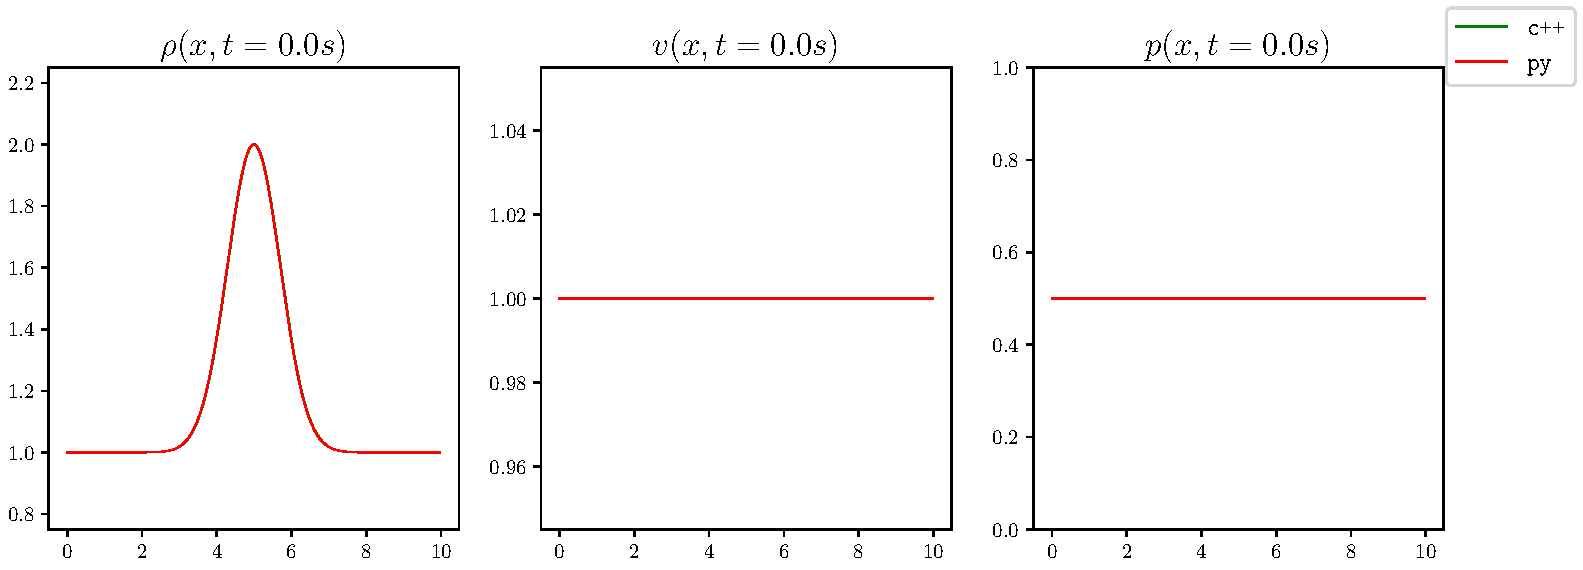
\includegraphics[width=1.1\linewidth]{../euler1D/plots_en_TDG/py_sin_claw/py_gauss199/1.pdf}
	\caption{Gráficas para $t=0.0\unit{\s}$}
\end{figure}

\begin{figure}[ht]
	\centering
	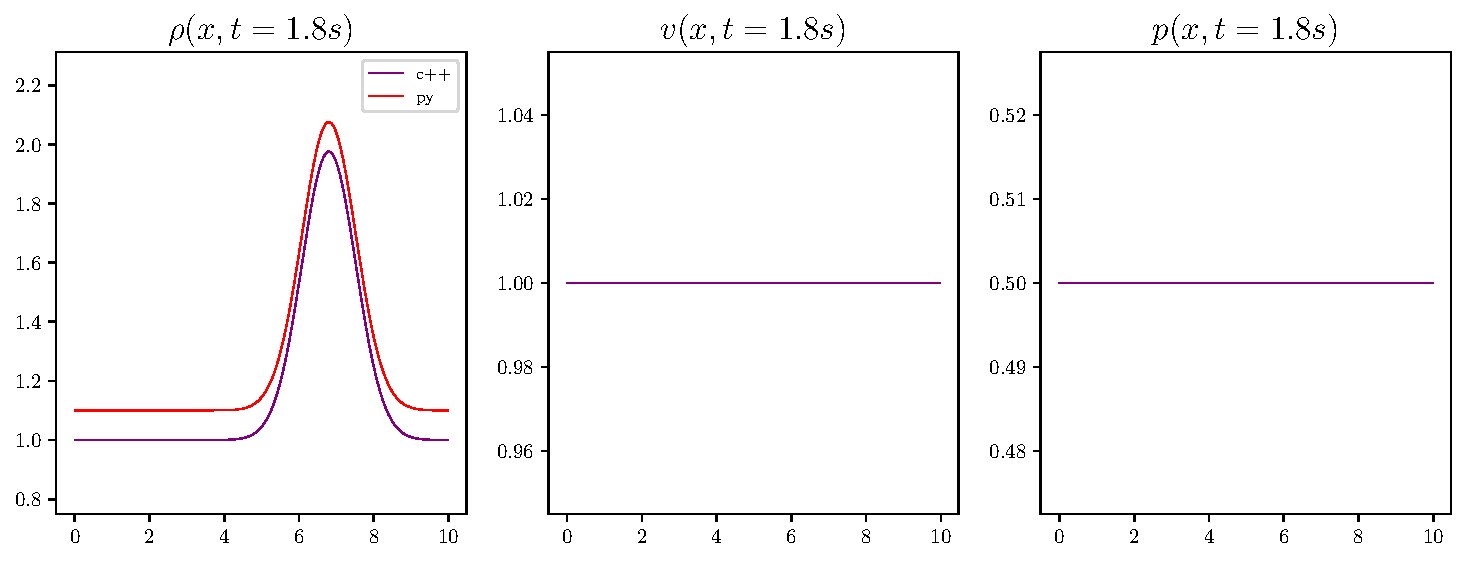
\includegraphics[width=1.1\linewidth]{../euler1D/plots_en_TDG/py_sin_claw/py_gauss199/4.pdf}
	\caption{Gráficas para $t=1.8\unit{\s}$}
\end{figure}

\begin{figure}[ht]
\centering
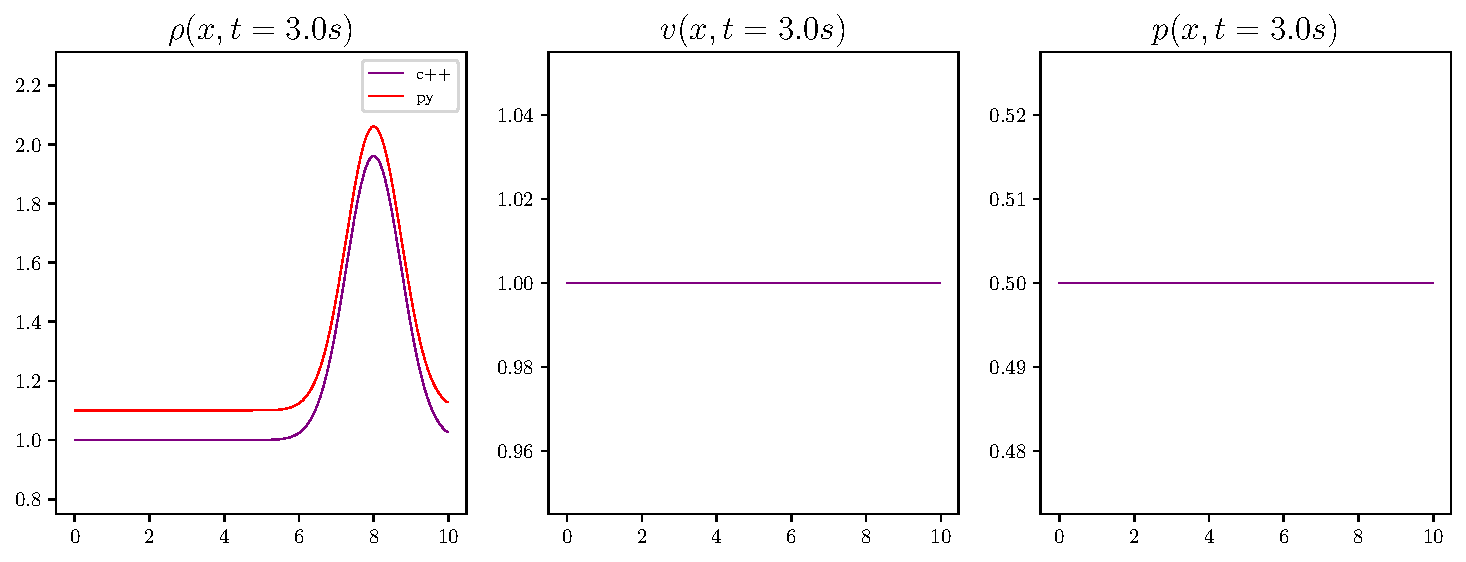
\includegraphics[width=1.1\linewidth]{../euler1D/plots_en_TDG/py_sin_claw/py_gauss199/6.pdf}
\caption{Gráficas para $t=3.0\unit{\s}$}
\label{fig:set-1-py-seg3}
\end{figure}

\begin{table}[ht]
	\large
	\centering
	\begin{tabular}{|l|l|l|l|}
		\hline
		Resultados & $\rho$ & $u$ & $p$ \\ \hline
		RMSE & 8.2e-03 & 0.0e+00 & 0.0e+00 \\ \hline
		Error máximo & 4.1e-02 & 0.0e+00 & 0.0e+00 \\ \hline
	\end{tabular}
	\caption{Comparativa de error entre simulaciones, primer conjunto de condiciones iniciales.}
	\label{tab:tabla-set-1}
\end{table}

\subsubsection{Discusión del primer conjunto de condiciones iniciales}
Se puede notar cómo la simulación de PyClaw sí mantiene la forma original de la campana gaussiana correspondiente a la densidad. En la figura \ref{fig:set-1-py-seg3} es apreciable que el máximo de las dos funciones difiere. Las funciones de velocidad y presión no presentan diferencias entre las dos simulaciones.


\subsection{Comparación del segundo conjunto de condiciones iniciales}
\subsubsection{Gráficas}
\begin{figure}[H]
	\centering
	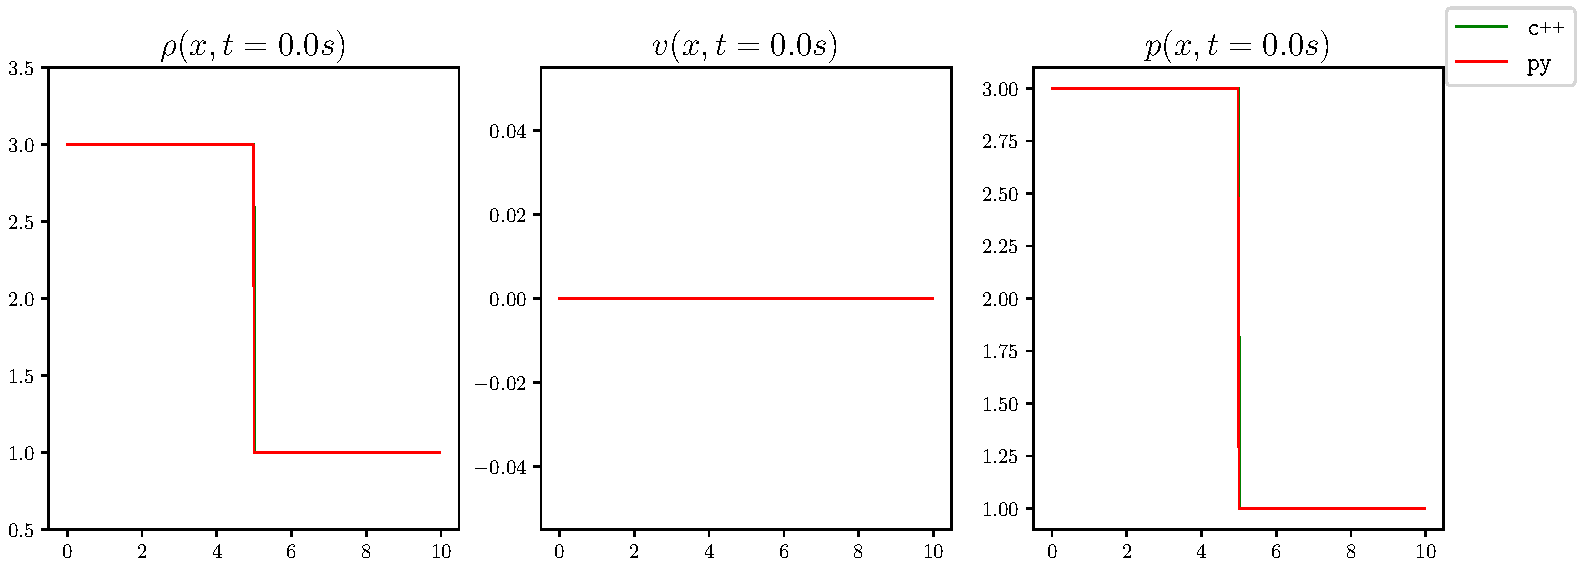
\includegraphics[width=1\linewidth]{../euler1D/plots_en_TDG/py_sin_claw/py_sod659/1.pdf}
	\caption{Gráficas para $t=0.0\unit{\s}$}
\end{figure}
\begin{figure}[H]
	\centering
	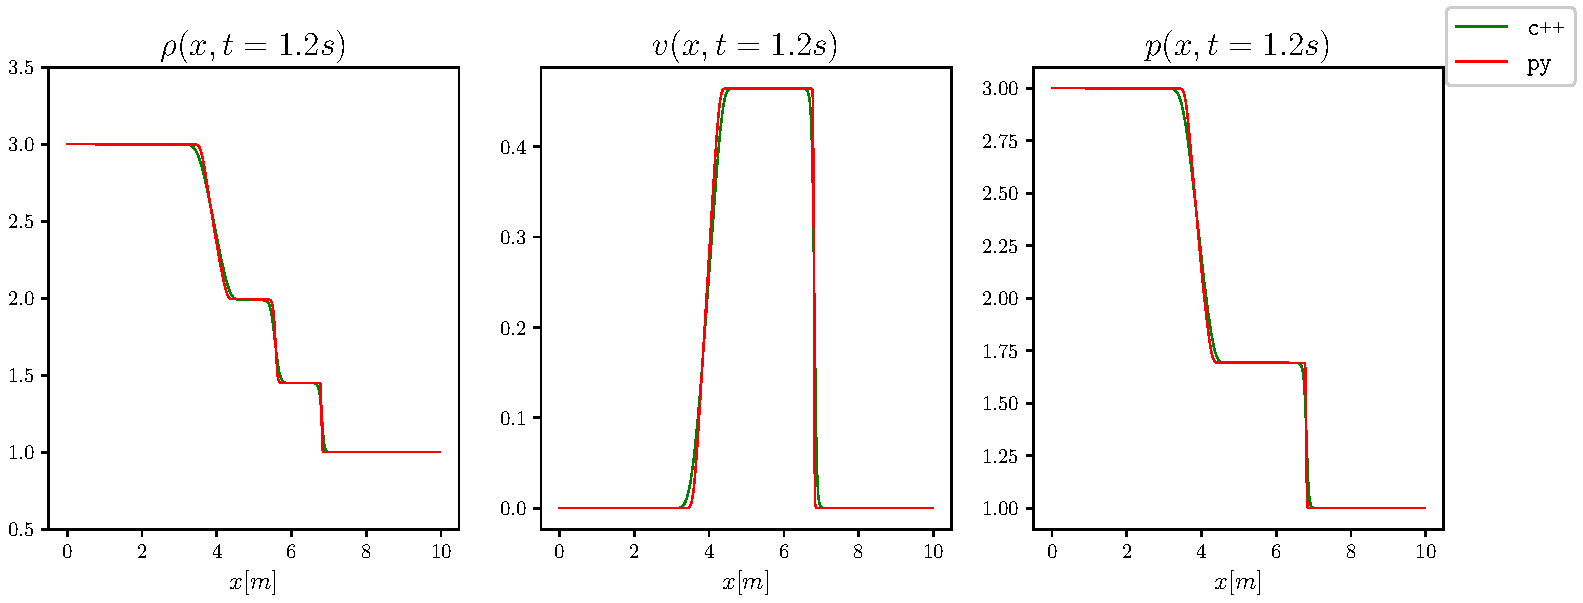
\includegraphics[width=1\linewidth]{../euler1D/plots_en_TDG/py_sin_claw/py_sod659/4.pdf}
	\caption{Gráficas para $t=1.2\unit{\s}$}
\end{figure}
\begin{figure}[H]
	\centering
	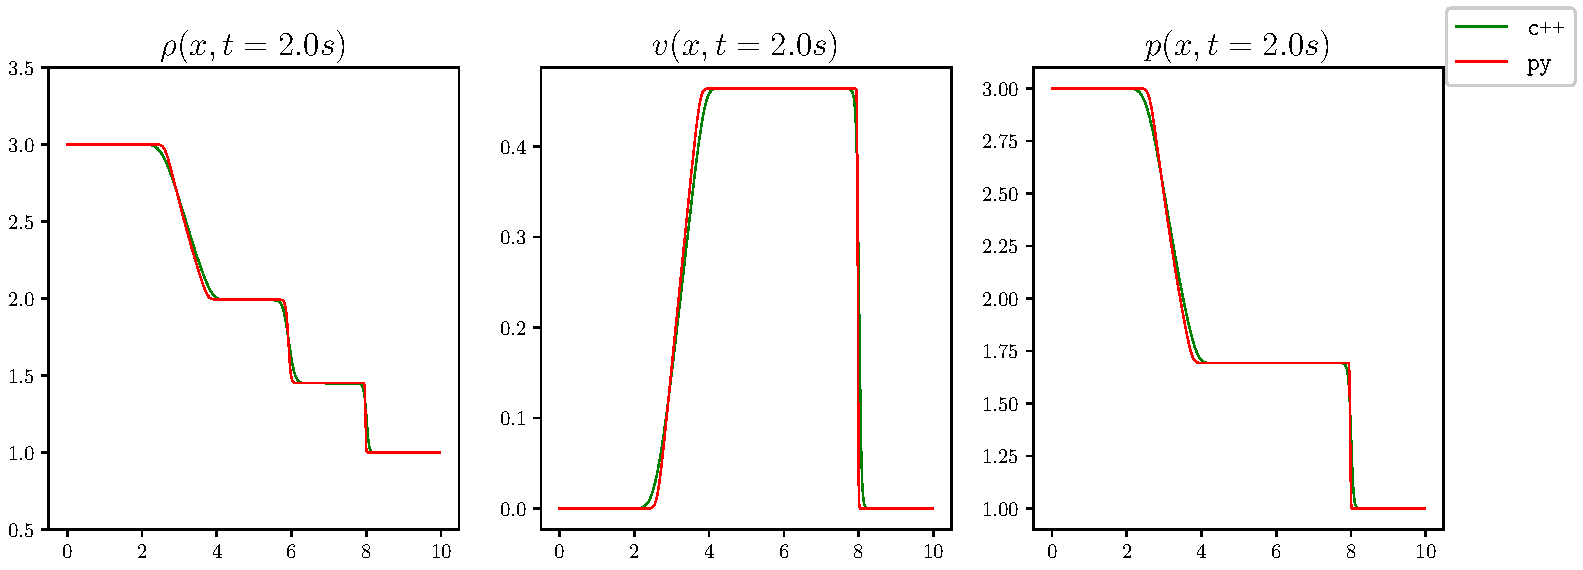
\includegraphics[width=1\linewidth]{../euler1D/plots_en_TDG/py_sin_claw/py_sod659/6.pdf}
	\caption{Gráficas para $t=3.0\unit{\s}$}
\end{figure}\vspace{\baselineskip}
\begin{table}[H]
	\large
	\centering
	\begin{tabular}{|l|l|l|l|} \hline
		Resultados & $\rho$ & $u$ & $p$ \\ \hline
		RMSE & 2.2e-02 & 1.4e-02 & 2.6e-02 \\ \hline
		Error máximo & 1.6e-01 & 1.7e-01 & 2.3e-01 \\ \hline
	\end{tabular}
	\caption{Comparativa de error entre simulaciones, segundo conjunto de condiciones iniciales.}
	\label{tab:tabla-set-2}
\end{table}
\vspace{3\baselineskip}
\subsubsection{Discusión del segundo conjunto de condiciones iniciales}
A través de la simulación con este conjunto de condiciones iniciales se destaca que las funciones producidas por PyClaw devuelven ondas de rarefacción distintas a las producidas por la simulación de C++, notando que poseen pendientes más pronunciadas cerca de las discontinuidades. Este hecho es más evidente al observar la evolución de la presión, ya que es la variable con el valor de RMSE más alto. Se puede inferir que esta diferencia se debe a los algoritmos de alta resolución implementados en PyClaw.

A través de esta simulación resalta que tanto el algoritmo implementado en C++ como los métodos de PyClaw capturan adecuadamente la velocidad de propagación de las ondas de choque y de rarefacción. Este hecho es importante dado que garantiza que los métodos implementados son conservativos.
\clearpage
%
\subsection{Comparación del tercer conjunto de condiciones iniciales}
\subsubsection{Gráficas}
\begin{figure}[H]
	\centering
	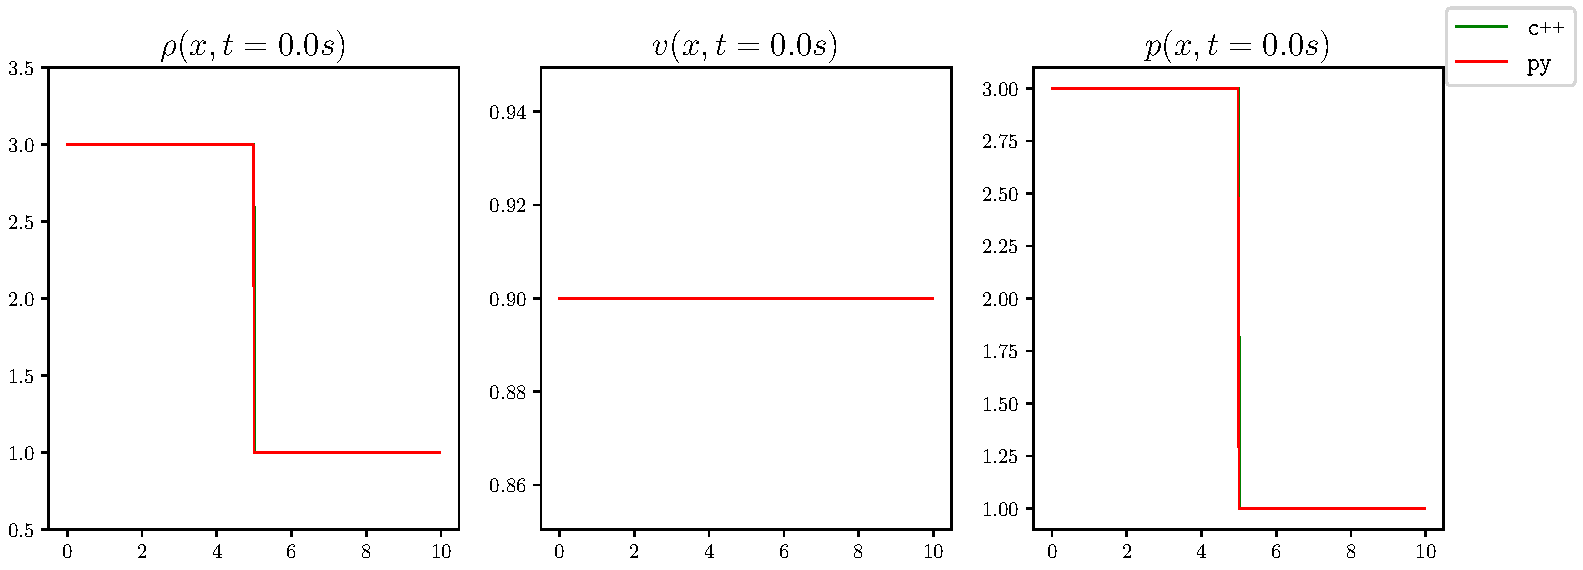
\includegraphics[width=1\linewidth]{../euler1D/plots_en_TDG/py_sin_claw/py_leveque518/1.pdf}
	\caption{Gráficas para $t=0.0\unit{\s}$}
\end{figure}
\begin{figure}[H]
	\centering
	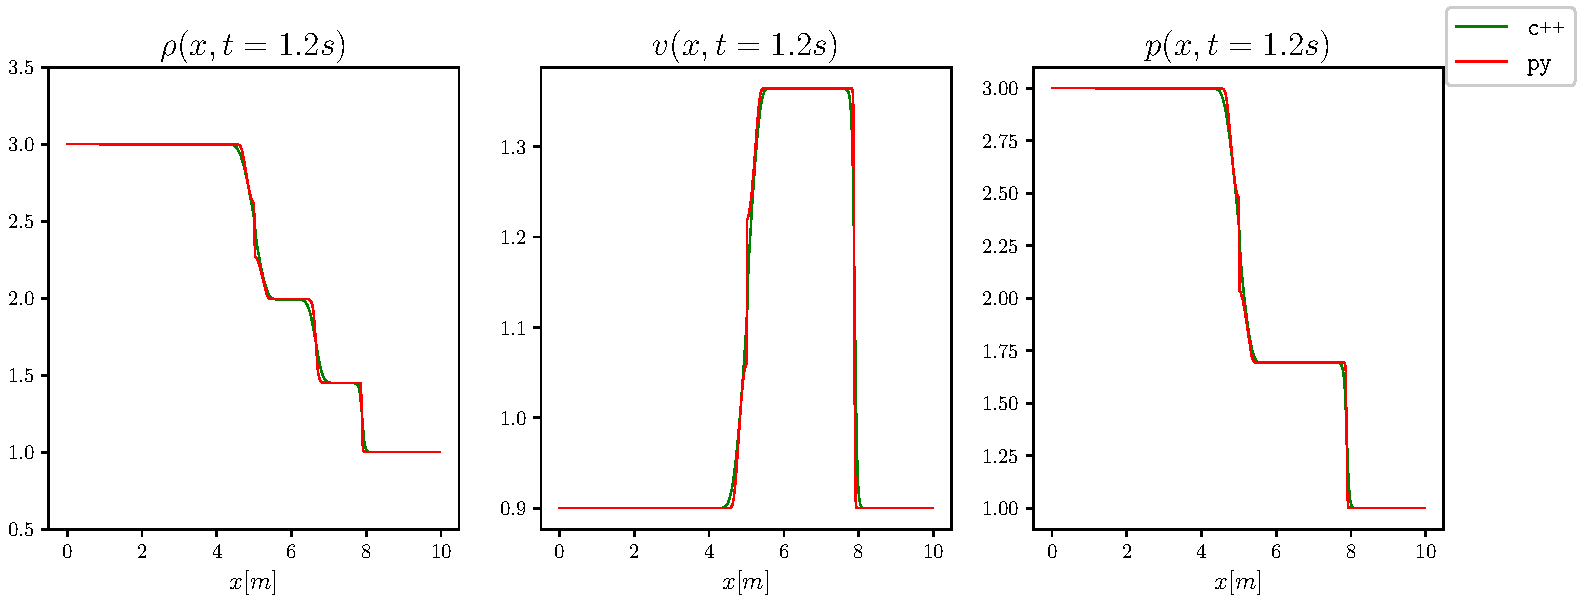
\includegraphics[width=1\linewidth]{../euler1D/plots_en_TDG/py_sin_claw/py_leveque518/4.pdf}
	\caption{Gráficas para $t=1.2\unit{\s}$}
\end{figure}
\begin{figure}[H]
	\centering
	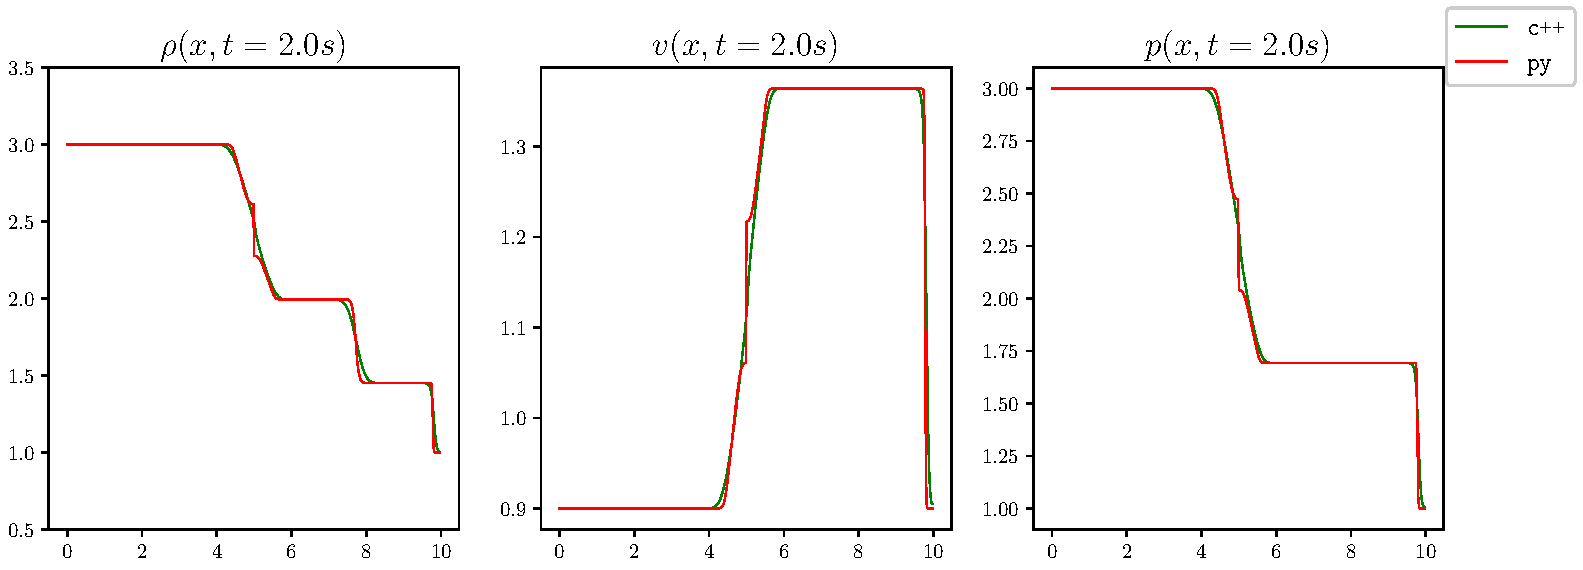
\includegraphics[width=1\linewidth]{../euler1D/plots_en_TDG/py_sin_claw/py_leveque518/6.pdf}
	\caption{Gráficas para $t=2.0\unit{\s}$}
\end{figure}
\begin{table}[H]
	\large
	\centering
	\begin{tabular}{|l|l|l|l|}
		\hline
		Resultados & $\rho$ & $u$ & $p$ \\ \hline
		RMSE & 2.5e-02 & 1.4e-02 & 2.6e-02 \\ \hline
		Error máximo & 2.5e-01 & 1.6e-01 & 3.2e-01 \\ \hline
	\end{tabular}
	\caption{Comparativa de error entre simulaciones, tercer conjunto de condiciones iniciales.}
\end{table}
\subsubsection{Discusión del tercer conjunto de condiciones iniciales}
En este conjunto de soluciones se expone una diferencia que ya había sido observada en los resultados de la simulación con C++ con la corrección de entropía y sin ésta (sección \ref{sec:set-3-cpp}). El algoritmo de PyClaw no considera la corrección de entropía en el esquema de Roe, a diferencia del programa escrito en C++, que sí tiene esta funcionalidad. Por estas razones, este conjunto de soluciones son las que presentan los mayores RMSE. Aunque los errores máximos encontrados no parecen alarmantes, si se dejara correr la simulación por más tiempo, se esperaría que el error aumentara considerablemente. 